\scanpage{4}

\mspage{2}
\deleted{$2i-1+2j-1=2(i+j-1)=\unsure{2n|n}$}

\margin{\uline{``Néron''}}
\uline{Th. 5} Soit $X$ Variété projective n.s. de dim $n$
\deleted{\unsure{même}}, $Z^i,Z'{}^j\in\mathcal Z^*(X)$
\inserted{de codim $i,j$, avec \deleted{\unsure{et}} $i+j=n$}
supposons que
\[
\zeta=Z\mathbin{.}Y\quad\text{et}\quad\zeta'=Z'\mathbin{.}Y
\]
soient alg. équiv. à $0$\inserted{\figure{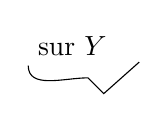
\begin{tikzpicture}\node(n){sur $Y$};\draw(n.south west) to[out=-90,in=180](.2,-.4)--(.4,-.6)--(.85,-.2);\end{tikzpicture}}}
[$Y$ section hyperplane\inserted{\figure{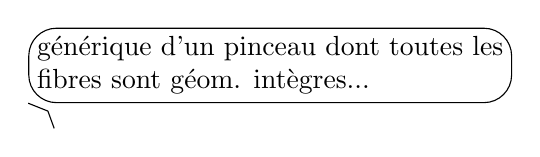
\begin{tikzpicture}
\node[draw,rounded corners=10pt,align=left,inner sep=3pt](n){générique d'un pinceau dont \deleted{\unsure{toutes}} les\\fibres sont géom. intègres...};
\draw(n.south west)--++(.25,-.1)--++(.08,-.22);
\end{tikzpicture}}}]; ils sont de codim \deleted{\unsure{en dim}}\inserted{$i,j$}, avec \deleted{$\dim Y=2m-1$}\inserted{$i+j=n=\dim Y+1$}
donc \deleted{\unsure{sont des}}\inserted{définissent des} éléments de $P^{\unsure{i}}(Y),P^{\unsure{j|0}}(Y)$ et par la forme de Néron--Tate [définie grâce à l'isomorphisme entre $P^{\unsure{i}}(Y)$ et $P^{\unsure{j|0}}(Y)$] on \deleted{alors} définit $\langle\zeta,\zeta'\rangle$. Ceci posé, on a \deleted{[au signe près ??]}
\[
\langle\zeta,\zeta'\rangle=(-1)^m Z\mathbin{.}Z'
\]

\margin{\figure{\begin{tikzpicture}
\node[draw,ellipse,rotate=28,align=left,inner sep=6pt]{\uline{N.B.} Sauf\\si $2i=2j=n$\\les deux mbres\\sont nuls\\par Lefschetz \unsure{au|en}\\\unsure{sens général|sens géométrique}};
\end{tikzpicture}}}
\margin{\figure{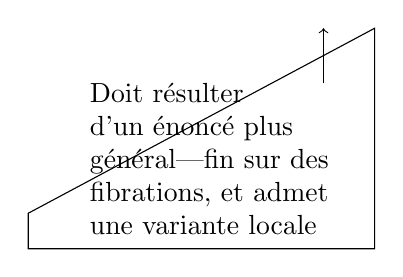
\begin{tikzpicture}
\draw(0,0)--(4.4,0)--(4.4,2.8)--(0,.45)--cycle;
\node[align=left,anchor=south] at(2.3,.05){Doit résulter\\d'un énoncé plus\\\unsure{général|fin} sur des\\fibrations, et admet\\une \uline{variante} locale};
\draw[->](3.75,2.1)--(3.75,2.8);
\end{tikzpicture}}}

\deleted{\uline{Cor.}}\inserted{\uline{Th. 6}}
Dans les conditions du th 5,
Si $2i\leq n-1$ $P^i(X)\mathbin{-}P^i(Y)$ est un \uline{isomorphisme}; \deleted{\unsure{et}} \uline{si $2i=n$}
Le \uline{facteur fixe} de $P^i(Y)$ est identique à l'image de $P^i(X)$;
\deleted{\unsure{Et} [\unsure{est égale à} $P^i(X)$]}
\inserted{\deleted{\unsure{pour|pair}}}
\deleted{\unsure{que} [Si \deleted{$2i\unsure{=|\leq}n$}\inserted{$n=2i$}, \unsure{si} $n$ pair et $i=\frac n2$]}
\deleted{Le noyau de $P^i(X)\mathbin{-}P^i(Y)$ est fini}
[Si \deleted{$\unsure{\leq}$} $2i\geq n+1$, $P^i(X)\mathbin{-}P^i(Y)$ est \inserted{\deleted{$2i\leq n+1$}\uline{surjectif}}]

\margin{\uline{``Lefschetz''}\figure{\begin{tikzpicture}\draw(0,0)--(0,3.6);\draw(.12,3.9)--(.12,4.7)--(.36,4.7);\end{tikzpicture}}}
\mspage{3}
